%%%%%%%%%%%%%%%%%%%%%%%%%%%%%%%%%%%%%%%%%%%%%%%%%%%%%%%%%%%%%%%%%%%%%%
%% CCADD (Current Computer-Aided Drug Design) - Research Article
%% Bentham Science Free Format Submission
%% v2: Fixed references, layout, structure, missing data
%% Date: 2026-10-19
%%%%%%%%%%%%%%%%%%%%%%%%%%%%%%%%%%%%%%%%%%%%%%%%%%%%%%%%%%%%%%%%%%%%%%

\documentclass[10pt,a4paper,twocolumn]{article}

\usepackage{times}
\usepackage{amsmath,amssymb}
\usepackage{graphicx}
\usepackage{booktabs}
\usepackage{multirow}
\usepackage{xcolor}
\usepackage{hyperref}
\usepackage{caption}
\usepackage{geometry}
\usepackage{placeins}
\usepackage{float}
\geometry{margin=2.0cm}

\setlength{\parindent}{0pt}
\setlength{\parskip}{6pt}

\begin{document}

%%%%%%%%%%%%%%%%%%%%%%%%%%%%%%%%%%%%%%%%%%%%%%%%%%%%%%%%%%%%%%%%%%%%%%
%% RUNNING TITLE (added per v2 review)
%%%%%%%%%%%%%%%%%%%%%%%%%%%%%%%%%%%%%%%%%%%%%%%%%%%%%%%%%%%%%%%%%%%%%%
\pagestyle{myheadings}
\markboth{Ren et al. / Contrastive Learning Reassessed for DTA}{Convergent-Protocol Reassessment of CL for DTA}

%%%%%%%%%%%%%%%%%%%%%%%%%%%%%%%%%%%%%%%%%%%%%%%%%%%%%%%%%%%%%%%%%%%%%%
%% TITLE
%%%%%%%%%%%%%%%%%%%%%%%%%%%%%%%%%%%%%%%%%%%%%%%%%%%%%%%%%%%%%%%%%%%%%%
\begin{center}
{\LARGE\bfseries Apparent Contrastive Learning Gains in Drug--Target Affinity Prediction Are Manufactured by Under-Converged Supervised Baselines: A Convergent-Protocol Reassessment}

\vspace{1em}

{\large Xiaoping Ren$^{1,*}$, Chaoya Sui$^{1}$, Xiaoyong Liu$^{1}$, Xiaoli Ren$^{1}$, Ling Tao$^{2}$, and Yan Zhang$^{3}$}

\vspace{0.5em}

\small
$^{1}$Chongqing Chemical Industry Vocational College, Chongqing 401228, China\\
$^{2}$Department of Oncology, The People's Hospital of Chongqing Liang Jiang New Area, Chongqing 401120, China\\
$^{3}$YaoPharma Co., Ltd., Chongqing 401121, China\\

\vspace{0.5em}
*Corresponding author: Xiaoping Ren (rxp613@gmail.com; Tel.: +86-15828596879)
\end{center}

\noindent\rule{\linewidth}{1pt}

\textbf{Keywords:} drug--target affinity; contrastive learning; graph neural network; reproducibility; training convergence; protocol sensitivity; benchmark

\noindent\rule{\linewidth}{1pt}

%%%%%%%%%%%%%%%%%%%%%%%%%%%%%%%%%%%%%%%%%%%%%%%%%%%%%%%%%%%%%%%%%%%%%%
%% STRUCTURED ABSTRACT (Bentham format: BACKGROUND/OBJECTIVE/METHODS/RESULTS/CONCLUSION)
%%%%%%%%%%%%%%%%%%%%%%%%%%%%%%%%%%%%%%%%%%%%%%%%%%%%%%%%%%%%%%%%%%%%%%
\vspace{1em}
\noindent\textbf{Abstract}

\noindent\textbf{BACKGROUND:} Contrastive learning (CL) has been reported to improve drug--target affinity (DTA) prediction, but these claims rest on short training budgets (500 epochs with early-stopping patience of 50) under which convergence of the pure supervised baseline was never verified. Whether reported CL gains are genuine improvements or artifacts of an under-converged reference is therefore unresolved.

\noindent\textbf{OBJECTIVE:} To test whether previously reported CL gains survive once the supervised baseline is trained to convergence, and to map the true effect of CL across encoder architectures, datasets, loss weights, and split protocols.

\noindent\textbf{METHODS:} We executed a pre-registered 2$\times$2 protocol-sensitivity design---training protocol (Config B: 500 epochs/patience 50 vs.\ Config C: 1{,}000 epochs/patience 150) crossed with condition (pure supervised E0 vs.\ CL E7, $\alpha=0.05$)---together with six-dose CL weight sweeps, scaffold splits, and cold-start splits, using 5--10 matched seeds. Convergence was audited from the selected epoch against the epoch ceiling; significance was assessed by paired $t$-tests (primary), Welch and Levene tests, Friedman repeated-measures tests, and Hedges' $g$ with Bonferroni/Benjamini--Hochberg correction.

\noindent\textbf{RESULTS:} Under Config C on KIBA ($n=10$), the supervised baseline (MSE 0.1381$\pm$0.0116; CI 0.8825) significantly outperforms CL (0.1495$\pm$0.0080; CI 0.8738): CL is 8.28\% worse on MSE (paired $p=0.0011$, $d_z=1.50$) and 0.98\% worse on CI ($p=0.0010$). On Davis with the GIN encoder ($n=10$), E0 (0.2032) and E7 (0.2000) do not differ significantly ($p=0.41$). The Davis dose--response ($n=5$) shows no CL weight significant after correction (Friedman $p=0.053$), whereas on KIBA $\alpha=0.5$ worsens MSE by 17.08\% (Bonferroni $p=0.0005$; Friedman $p=0.015$). With the weaker GAT encoder on Davis ($n=5$), CL reduces MSE by 10.19\% (0.2617$\to$0.2351; $p=0.0005$; 5/5 seeds), yet the CL-trained GAT still does not match the GIN baseline (0.2021). On scaffold splits no significant difference survives ($p=0.30$), and under cold splits warm-validation model selection fails (18$\times$ validation--test disconnect).

\noindent\textbf{CONCLUSION:} In the strongest prior case (KIBA), reported CL gains are manufactured by an under-converged supervised baseline and reverse sign under a convergent protocol. CL offers no cross-benchmark robust benefit; its effect changes sign with encoder and dataset. Convergence auditing and protocol control are therefore mandatory before attributing gains to auxiliary losses in DTA and comparable molecular regression tasks.

\noindent\rule{\linewidth}{1pt}

%%%%%%%%%%%%%%%%%%%%%%%%%%%%%%%%%%%%%%%%%%%%%%%%%%%%%%%%%%%%%%%%%%%%%%
%% 1. INTRODUCTION
%%%%%%%%%%%%%%%%%%%%%%%%%%%%%%%%%%%%%%%%%%%%%%%%%%%%%%%%%%%%%%%%%%%%%%
\section{INTRODUCTION}

Drug--target affinity (DTA) prediction is a central task in computer-aided drug design, enabling rapid estimation of binding strength between candidate compounds and protein targets \cite{ozturk2018deepdta,nguyen2021graphdta}. Accurate DTA models can accelerate lead identification, drug repurposing, and virtual screening campaigns, reducing the cost and timeline of early-stage drug discovery \cite{vamathevan2019applications,huang2022artificial}. In the context of virtual screening, DTA prediction models rank compound libraries by predicted binding affinity, enabling experimental validation of top-ranked candidates \cite{abbasi2021deepdti,gorgulla2020virtual,tsubaki2019cpi}. Complementarily, structure-based docking methods such as AutoDock4 \cite{morris2009autodock4} and AutoDock Vina \cite{trott2010vina} estimate binding poses from protein structures. Recent advances in deep learning have substantially improved prediction accuracy, with models achieving concordance indices above 0.85 on standard benchmarks \cite{bagherian2021ml,chen2016dti}.

Deep learning approaches for DTA prediction have evolved along two major axes. \textbf{Sequence-based models} such as DeepDTA \cite{ozturk2018deepdta}, WideDTA \cite{ozturk2019widedta}, and DeepConv-DTI \cite{lee2019deepconvdti} employ convolutional encoders to process drug SMILES strings and protein sequences. These models treat molecules as strings, which simplifies input representation but potentially loses structural information. \textbf{Graph-based models} such as GraphDTA \cite{nguyen2021graphdta}, DGraphDTA \cite{jiang2021dgraphdta}, and MolTrans \cite{huang2021moltrans} represent drugs as molecular graphs and apply graph neural networks (GNNs) \cite{xu2019powerful,velickovic2018gat,kipf2017semi,gilmer2017mpnn,schutt2018schnet,dwivedi2023benchmark,hamilton2017graphsage,ying2018diffpool} to preserve topological information. This graph-based approach captures molecular structure more faithfully and has achieved state-of-the-art performance on multiple benchmarks. Additional architectures including MONN \cite{li2020monn}, DeepCDA \cite{abbasi2020deepcda}, AttentionDTA \cite{zhao2023attentiondta}, DeepAffinity \cite{karimi2019deepaffinity}, and TransformerCPI \cite{chen2020transformercpi} have further pushed performance boundaries through attention mechanisms and interaction-aware modeling. Recent comprehensive benchmarks \cite{bagherian2021ml,chen2016dti} have systematically compared these approaches, establishing strong supervised baselines on standard datasets such as Davis \cite{davis2011predicting} and KIBA \cite{tang2014kiba}.

Despite these advances, current DTA models face limitations in generalization to novel chemical space and understudied protein targets. Standard evaluation protocols use random splits where test drugs and targets overlap with training data, leading to optimistic performance estimates \cite{pahikkala2015toward,park2012flaws}. Cold-start scenarios---where test sets contain entirely unseen drugs or targets---better reflect real-world drug discovery challenges but remain underexplored. Scaffold split evaluation \cite{bemis1996properties}, which ensures no shared molecular frameworks between training and test sets, provides a rigorous assessment of out-of-distribution generalization but is rarely applied in DTA studies. Recent work has begun addressing these gaps through few-shot learning and out-of-distribution detection, but systematic characterization of model behavior under cold-start conditions remains lacking.

Contrastive learning (CL) has emerged as a powerful self-supervised paradigm in molecular representation learning. GraphCL \cite{you2020graphcl} introduced graph augmentations for molecular contrastive learning, MolCLR \cite{wang2022molclr} applied CL to molecular property prediction, and 3D Infomax \cite{stark2022contrastive} leveraged geometric information for pre-training. Other notable methods include InfoGraph \cite{sun2019infograph}, GCC \cite{qiu2020gcc}, GraphMAE \cite{hou2022graphmae}, SimGRACE \cite{xia2022simgrace}, JOAO \cite{you2021joao}, and GROVER \cite{rong2020grover}. These methods have demonstrated success in molecular property prediction and other classification tasks, motivating their extension to DTA regression \cite{wu2023selfsupervised,forooghi2026survey,deng2026review,david2020molecular}. Recent reviews have highlighted the potential of contrastive learning for molecular representation but noted the lack of systematic evaluation in regression settings \cite{jaiswal2021survey}.

A measurement pitfall cuts across this literature. Apparent gains for an auxiliary objective can be manufactured when the reference model is under-trained: equal epoch budgets do not imply equal optimization, and stopping rules tuned for one condition can prematurely truncate another \cite{lones2021pitfalls,damour2020underspecification}. This confound is particularly dangerous for paired comparisons such as ``supervised baseline vs.\ supervised + CL'', because any under-convergence of the baseline is read as a gain for the added loss. In the DTA CL studies cited above---and in our own earlier reports---headline numbers were obtained under a 500-epoch budget with early-stopping patience of 50, yet training audits show pure supervised runs still improving at the epoch ceiling (best checkpoint at epoch 995/1000). The convergence of the very baseline against which CL was scored was therefore never established, and the sign and magnitude of the reported effects are correspondingly suspect.

Several recent works have explored contrastive learning specifically for DTA prediction. CSGNN \cite{zhao2021csgnn} proposed contrastive self-supervised graph learning for molecular interaction prediction. GraphCL-DTA \cite{yang2024graphcl} incorporated molecular semantics into contrastive objectives. CSCo-DTA \cite{wang2024csco} integrated multi-scale features with cross-scale contrastive learning. MLC-DTA \cite{zheng2025mlc} combined multi-level contrastive learning with equivariant GNNs. Collaborative CL approaches \cite{tian2024drug} have further explored adaptive sampling strategies for DTA. Re-examined through the measurement lens above, these studies share three critical limitations: (i) the supervised comparator is assumed rather than verified to be converged, leaving reported gains unidentified as between the auxiliary loss and the training protocol; (ii) training protocol and learning condition are varied together, so protocol sensitivity of the claimed effect is never measured; and (iii) model selection by warm (entity-overlapping) validation performance is used under cold-start and scaffold splits without checking whether that selection mechanism remains valid out of distribution. Whether CL benefits transfer to genuinely novel chemical space remains open for the same reason.

In this work, we resolve the confound directly rather than add another CL variant. We hold model, data, and all optimizer hyperparameters fixed, and vary only the training protocol---a pre-registered 2$\times$2 design crossing protocol (Config B, 500 epochs/patience 50, vs.\ Config C, 1{,}000 epochs/patience 150) with condition (E0 vs.\ CL E7)---then map the convergent-protocol effect across CL weights, two encoders (GIN, GAT), two datasets (Davis, KIBA), and standard, scaffold, and cold-start splits. Our contributions are: (i) a protocol-sensitivity demonstration that the largest previously reported CL gain (+61.16\% on KIBA) collapses and reverses to a significant 8.28\% \emph{degradation} once the supervised baseline converges ($n=10$, paired $p=0.0011$); (ii) a convergent-protocol effect map establishing an encoder$\times$dataset interaction---null on GIN/Davis, significantly positive on GAT/Davis ($+10.19\%$), significantly negative on GIN/KIBA---with no cross-benchmark robust benefit; (iii) a methodological analysis showing that warm-validation model selection fails under cold splits (18$\times$ validation--test disconnect); and (iv) a convergence-audit checklist and conditional deployment guidelines for auxiliary-loss claims in DTA and comparable molecular regression tasks.

%%%%%%%%%%%%%%%%%%%%%%%%%%%%%%%%%%%%%%%%%%%%%%%%%%%%%%%%%%%%%%%%%%%%%%
%% 2. MATERIALS AND METHODS
%%%%%%%%%%%%%%%%%%%%%%%%%%%%%%%%%%%%%%%%%%%%%%%%%%%%%%%%%%%%%%%%%%%%%%
\section{MATERIALS AND METHODS}

\subsection{Datasets}

\textbf{Davis Dataset} \cite{davis2011predicting}: Contains 30,056 drug--target pairs (68 drugs $\times$ 442 targets) with $pK_d$ values ranging from [5.0, 10.8]. The dataset is enriched for kinase families and approved drugs.

\textbf{KIBA Dataset} \cite{tang2014kiba}: Contains 118,254 drug--target pairs from 2,111 drugs and 229 targets with KIBA scores ranging from [0.0, 17.2]. After filtering 9 invalid zero-affinity samples from the original 118,263 pairs, KIBA provides a larger-scale benchmark with broader chemical space coverage. Both datasets were derived from their original publications \cite{davis2011predicting,tang2014kiba} and are publicly available through the Therapeutics Data Commons (TDC) \cite{huang2021tdc}.

\subsection{Model Architecture}

We implement two drug encoder variants under identical protocols. \textbf{GIN}: Three Graph Isomorphism Network layers \cite{xu2019powerful} with learnable MLPs and global sum pooling (498,177 parameters). \textbf{GAT}: Three Graph Attention Network layers \cite{velickovic2018gat} with 4 attention heads and concatenation (521,345 parameters). Both take 40-dimensional atom features---comprising atomic number, degree, formal charge, hybridization type (one-hot, 5 categories), hydrogen count, ring membership, aromaticity, atomic mass, total valence, radical electrons (10 scalar features, each normalized to [0,1]), plus a 25-bin one-hot encoding of atomic number (bins of width 5, covering Z=0--125), and a substructure membership flag---and output 128-dimensional graph representations. The protein encoder is a 1D-CNN (three convolutional layers with kernel sizes 3/5/7, global max pooling, 128-dimensional output) operating on integer-encoded amino acid sequences (vocabulary: 20 standard amino acids + unknown + padding token; maximum sequence length 1000 residues, with truncation for longer sequences and padding for shorter ones). Drug and protein representations are concatenated (256-dim) and fed into an MLP predictor (256$\to$512$\to$128$\to$1) with ReLU and dropout ($p=0.3$). For comparison, we also implement DeepDTA \cite{ozturk2018deepdta} (1D-CNN, 1.01M params) and GraphDTA-GAT \cite{nguyen2021graphdta} (GAT+1D-CNN, 946K params) as baseline methods.

\subsection{Contrastive Loss Formulation}

The total training loss combines MSE with three contrastive components:
\begin{equation}
\mathcal{L} = \mathcal{L}_{\text{MSE}} + \alpha \cdot \mathcal{L}_{\text{InfoNCE}} + \beta \cdot \mathcal{L}_{\text{uniform}} + \gamma \cdot \mathcal{L}_{\text{cross}}
\end{equation}

\textbf{InfoNCE Loss} \cite{oord2018representation,chen2020simclr,he2020moco,gutmann2010nce}: Maximizes agreement between two augmented views $z_d^1, z_d^2$ of the same drug graph:
\begin{equation}
\mathcal{L}_{\text{InfoNCE}} = -\log \frac{\exp(\text{sim}(z_d^1, z_d^2) / \tau)}{\sum_{k=1}^{2B} \exp(\text{sim}(z_d^1, z_d^k) / \tau)}
\end{equation}
where $\text{sim}(u, v) = u^T v / (\|u\| \|v\|)$ is cosine similarity, $\tau = 0.1$ is temperature, and $B$ is batch size.

\textbf{Uniformity Loss} \cite{wang2020understanding}: Encourages uniform representation distribution on the hypersphere:
\begin{equation}
\mathcal{L}_{\text{uniform}} = \log \mathbb{E}_{z, z' \sim p_{\text{data}}} \left[\exp(-2\|z - z'\|^2)\right]
\end{equation}

\textbf{Cross-Modal Loss}: Aligns drug and protein representations by treating $(z_d, z_p)$ pairs from the same drug--target pair as positives:
\begin{equation}
\mathcal{L}_{\text{cross}} = -\log \frac{\exp(\text{sim}(z_d, z_p) / \tau)}{\sum_{k=1}^{B} \exp(\text{sim}(z_d, z_p^k) / \tau)}
\end{equation}

\subsection{Training Protocols and Hyperparameters}

We implemented three drug-side augmentation strategies during protocol development: (1) \textbf{Gaussian Noise}: add Gaussian noise to atom features ($X' = X + \epsilon$, $\epsilon \sim \mathcal{N}(0, 0.01 I)$); (2) \textbf{Random Node Masking}: randomly mask 20\% of nodes; (3) \textbf{Substructure-Aware Masking}: protect chemically important substructures (identified using RDKit \cite{landrum_rdkit} and ECFP fingerprints \cite{rogers2010ecfp}) and mask only non-substructure atoms. All experiments in the present reassessment use Gaussian noise exclusively, so augmentation identity is never confounded with the protocol or condition comparisons.

\textbf{Common (frozen) hyperparameters.} Adam optimizer \cite{kingma2015adam}, learning rate $5 \times 10^{-4}$, weight decay $1 \times 10^{-4}$, batch size 512, ReduceLROnPlateau scheduler (factor 0.5, patience 30 epochs without validation improvement). The contrastive temperature is fixed at $\tau=0.1$ and $\beta=\gamma=0$ throughout.

\textbf{Two training protocols.} The study is organized around two protocols that differ only in the epoch budget:
\begin{itemize}
\item \textbf{Config B (under-budgeted protocol):} maximum 500 epochs; early-stop patience 150.
\item \textbf{Config C (convergent protocol):} maximum 1{,}000 epochs; early-stop patience 150.
\end{itemize}
The scheduler patience (30) and early-stop patience (150) are identical across protocols; only \texttt{max\_epochs} changes (500 $\to$ 1{,}000), so any difference between protocols is attributable to training budget rather than to optimizer behavior.

\textbf{Model selection.} In all protocols we retain the checkpoint with the lowest validation-set MSE and evaluate it on the test set; early stopping terminates a run after 150 consecutive epochs without validation improvement. Under Config B, runs that terminate at the epoch cap with best epoch at or near the cap did not, in fact, early-stop and are flagged as \textit{ceiling-hitting} (best epoch $\geq 480$ at a 500-epoch cap; $\geq 980$ at a 1{,}000-epoch cap), i.e., the selection criterion never fired and the restored checkpoint is the final one. Hyperparameter choices, including $\alpha$, are made on validation data only.

\textbf{Splits.} We use: (i) the standard random 70/10/20 split; (ii) a Bemis--Murcko scaffold split with no shared scaffold between train and test; and (iii) three entity-disjoint cold splits (cold-drug, cold-target, cold-both) in which the corresponding test entities are absent from train and validation.

\textbf{Seeds and $\alpha$ grids.} Standard-split GIN experiments use ten matched seeds on both datasets: 42, 7, 123, 456, 789, 101, 202, 303, 404, 505. GAT Davis and the Davis and KIBA dose--response experiments use five matched seeds (42, 7, 123, 456, 789); scaffold experiments use 42, 7, 123, 2024, 3407. Under Config C, $\alpha$ is scanned over $\{0.01, 0.02, 0.05, 0.1, 0.2, 0.5\}$ on Davis and over $\{0, 0.05, 0.5\}$ on KIBA.

\subsection{Evaluation Metrics and Statistical Testing}

We report mean squared error (MSE, primary metric) and Concordance Index (CI, standard pairwise counting), computed on the test set, as mean $\pm$ sample standard deviation over seeds. Because every comparison uses the same seeds for both conditions, the primary inference is the \textbf{paired two-sided Student $t$-test} over matched seed-level differences, reported together with the paired standardized mean difference $d_z$ (mean difference divided by the standard deviation of the paired differences) and a 95\% confidence interval (CI95) for the mean difference. As an unpaired robustness check we additionally compute the Welch $t$-test; equality of variances is checked with Levene's test. As a between-group standardized effect we report Hedges' $g$ \cite{hedges1981estimation} with the small-sample correction $J = 1 - 3/(4n - 9)$. Magnitudes follow Cohen's conventions \cite{cohen1988statistical}: small ($|g| \approx 0.2$), medium ($0.5$), large ($0.8$).

\textbf{Multiple-comparison and trend tests.} Within a dose--response family we apply Bonferroni correction (thresholds $0.05/6$ for the six Davis doses and $0.05/3$ for the three KIBA comparisons); the step-down Holm procedure \cite{holm1979simple} is used as a more powerful alternative where indicated. Overall dose effects are tested with the Friedman $\chi^2$ repeated-measures test, which respects the matched-seed design without assuming normality, and monotonic trends are summarized by Spearman's $\rho$. Where fewer than four dose levels are available, the asymptotic Spearman $p$-value is not valid: we report instead the exact two-sided permutation $p$-value (for three perfectly monotone levels, $p = 2/3! = 0.333$) and base monotonicity claims on the Friedman and paired tests.

\subsection{Computational Details and AI Tool Disclosure}

All experiments were conducted on NVIDIA RTX 3090 GPUs (24GB VRAM, CUDA 13.0) with Python 3.10.12, PyTorch 2.14.1 \cite{paszke2019pytorch}, PyTorch Geometric 2.8.1 \cite{fey2019pyg}, and RDKit 2021.09.2 \cite{landrum_rdkit}. The authors used Claude Code (Anthropic) solely for language editing, code debugging, and statistical analysis script development; all scientific content, experimental data, and conclusions are the authors' own.

%%%%%%%%%%%%%%%%%%%%%%%%%%%%%%%%%%%%%%%%%%%%%%%%%%%%%%%%%%%%%%%%%%%%%%
%% 3. RESULTS AND DISCUSSION
%%%%%%%%%%%%%%%%%%%%%%%%%%%%%%%%%%%%%%%%%%%%%%%%%%%%%%%%%%%%%%%%%%%%%%
%%%%%%%%%%%%%%%%%%%%%%%%%%%%%%%%%%%%%%%%%%%%%%%%%%%%%%%%%%%%%%%%%%%%%%
%% 3. RESULTS AND DISCUSSION
%% V9 rewrite (Tasks 3.3.1/3.3.3, 2026-11-12): built around the
%% 2x2 protocol-sensitivity design; all Config B-era claims replaced.
%%%%%%%%%%%%%%%%%%%%%%%%%%%%%%%%%%%%%%%%%%%%%%%%%%%%%%%%%%%%%%%%%%%%%%
\section{RESULTS AND DISCUSSION}

We present results in three parts. First, a controlled 2$\times$2 design isolates the effect of the training-budget protocol (Config B, 500 epochs, vs.\ Config C, 1{,}000 epochs) crossed with the learning condition (pure supervised E0 vs.\ contrastive E7); this is the study's primary contribution. Second, under the convergent Config C, we map the contrastive effect across two encoders, two benchmarks, and a full $\alpha$ dose range. Third, we document and diagnose a methodological failure of the standard warm-validation selection mechanism under cold and scaffold splits. Every number below is taken from per-run result files; sources are named in each table note, and full batch provenance is given in Supplementary Files S3--S4.

\subsection{Protocol Sensitivity: A Controlled 2$\times$2 Design}

\textbf{Motivating audit.} Before re-running experiments, we audited convergence under Config B by inspecting the selected epoch of each run. The result was unambiguous: on KIBA, all ten supervised E0 runs terminated at the 500-epoch budget with best epochs between 470 and 500 (eight of ten at $\geq 488$), and the five E7 runs selected epochs 441--497; on Davis, seven of ten E0 runs selected epochs $\geq 483$ (range 416--491) and E7 runs reached 344--491. The early-stopping criterion (patience 150) therefore rarely fired: most ``selected'' checkpoints were simply the final checkpoint of a truncated run. A direct single-seed probe quantified the consequence---KIBA E0 seed 42 moved from test MSE 0.1728 at 500 epochs to 0.1525 at 1{,}000 epochs (an 11.8\% improvement, best epoch 995), a budget effect several times larger than any reported CL gain. Figure~\ref{fig:v9_1} schematizes the resulting design.

% ============================================================================
% V9 Phase 3 auto-generated tables
% Generated: 2026-11-12T03:28:27.816153
% Goal: replace all Config B tables in main_ccadd.tex with Config C real results
% Method: values transcribed by v9_phase3_generate_tables.py from V9 analysis JSONs only
% ============================================================================

\begin{table*}[!t]
\caption{Main results under the convergent protocol (Config C: 1{,}000 epochs, LR patience 30, early-stop patience 150; all other hyperparameters frozen). E7: InfoNCE CL with $\alpha=0.05$, $\tau=0.1$, noise augmentation, $\beta=\gamma=0$. Values are mean$\pm$sample std; gain is E7 relative to E0 (positive = CL better); $p$ is the paired two-sided t-test over matched seeds; $d_z$ is the paired standardized mean difference.}
\label{tab:main_results}
\centering
\begin{tabular}{llccccccc}
\toprule
Dataset & Encoder ($n$) & E0 MSE & E7 MSE & MSE gain & paired $p$ & $d_z$ & E0 CI & E7 CI \\
\midrule
Davis & GIN (10) & 0.2032$\pm$0.0078 & 0.2000$\pm$0.0062 & +1.54\% & 0.4067 & -0.28 & 0.8951 & 0.8945 \\
Davis & GAT (5) & 0.2617$\pm$0.0060 & 0.2351$\pm$0.0061 & +10.19\%$^{***}$ & 0.0005 & -4.69 & 0.8815 & 0.8838 \\
KIBA & GIN (10) & 0.1381$\pm$0.0116 & 0.1495$\pm$0.0080 & -8.28\%$^{**}$ & 0.0011 & +1.50 & 0.8825 & 0.8738 \\
\bottomrule
\end{tabular}
\par\smallskip
\footnotesize $^{*}p<0.05$, $^{**}p<0.01$, $^{***}p<0.001$ (uncorrected paired p; family-wise claims are assessed in the dose--response tables and in Decision Gate A). Sources: \texttt{v9\_phase2p1\_davis\_stats.json}, \texttt{v9\_phase2p5\_gat\_stats.json}, \texttt{v9\_decision\_gate\_a.json}.
\end{table*}

\begin{table*}[!t]
\caption{Protocol sensitivity (2$\times$2 design): training protocol (Config B vs.\ Config C) crossed with condition (E0 vs.\ E7). Same model, same data, same optimizer hyperparameters; only the training budget and patience change. KIBA rows use the same five matched seeds; Davis rows use ten seeds. Positive gain = CL better; $p$ = paired t-test.}
\label{tab:protocol_sensitivity}
\centering
\begin{tabular}{llcccc}
\toprule
Dataset & Protocol & E0 MSE & E7 MSE & MSE gain & paired $p$ \\
\midrule
KIBA & B (500ep/p150) & 0.1497$\pm$0.0157 & 0.1476$\pm$0.0049 & +1.38\% & 0.7612 \\
KIBA & C (1000ep/p150) & 0.1366$\pm$0.0068 & 0.1473$\pm$0.0030 & -7.89\% & 0.0610 \\
\midrule
Davis & B (500ep/p150) & 0.2036$\pm$0.0044 & 0.1989$\pm$0.0069 & +2.33\% & 0.1289 \\
Davis & C (1000ep/p150) & 0.2032$\pm$0.0078 & 0.2000$\pm$0.0062 & +1.54\% & 0.4067 \\
\bottomrule
\end{tabular}
\par\smallskip
\footnotesize On KIBA the E7 mean is essentially protocol-invariant ($\sim$0.147--0.148); it is the E0 baseline that improves from 0.1497 to 0.1366 when trained to convergence, flipping the comparison sign. On Davis the E0 mean is nearly unchanged across protocols; protocol sensitivity is itself dataset-dependent and is strongest on KIBA. Sources: \texttt{v9\_phase0p3\_statistical\_tests.json}, \texttt{v9\_phase2p4\_kiba\_dose.json}, \texttt{v9\_phase2p1\_davis\_stats.json}.
\end{table*}

\begin{table*}[!t]
\caption{Davis dose--response under Config C (GIN, $n=5$ matched seeds). Gain is relative to $\alpha=0$ (positive = CL better); $p$ is the paired t-test. Bonferroni threshold $0.05/6=0.0083$; no dose reaches it.}
\label{tab:davis_dose}
\centering
\begin{tabular}{ccccc}
\toprule
$\alpha$ & MSE & gain & paired $p$ & Bonf sig. \\
\midrule
0 & 0.2021$\pm$0.0109 & — & — & — \\
0.01 & 0.1996$\pm$0.0049 & +1.21\% & 0.4601 & No \\
0.02 & 0.1954$\pm$0.0043 & +3.28\% & 0.3681 & No \\
0.05 & 0.1993$\pm$0.0031 & +1.36\% & 0.6353 & No \\
0.1 & 0.2027$\pm$0.0042 & -0.32\% & 0.8993 & No \\
0.2 & 0.2074$\pm$0.0068 & -2.62\% & 0.4293 & No \\
0.5 & 0.2072$\pm$0.0039 & -2.55\% & 0.2492 & No \\
\bottomrule
\end{tabular}
\par\smallskip
\footnotesize Friedman $\chi^2$ (7 levels, repeated measures): 12.429, $p=0.0531$ (borderline; not claimed significant). Spearman trend: $\rho=+0.64$, $p=0.1194$. Source: \texttt{v9\_phase2p3\_dose\_response.json}.
\end{table*}

\begin{table*}[!t]
\caption{KIBA dose--response under Config C (GIN, $n=5$ matched seeds). Three paired comparisons with Bonferroni threshold $0.05/3=0.0167$. Mean difference $>0$ = higher $\alpha$ worse (MSE).}
\label{tab:kiba_dose}
\centering
\begin{tabular}{lccccc}
\toprule
Comparison & mean diff & 95\% CI & $p$ & $d_z$ & Bonf sig. \\
\midrule
0.05 vs 0 & +0.0108 & [-0.0008,+0.0223] & 0.0610 & +1.16 & No \\
0.5 vs 0 & +0.0233 & [+0.0172,+0.0294] & 0.0005 & +4.73 & Yes \\
0.5 vs 0.05 & +0.0126 & [+0.0046,+0.0205] & 0.0116 & +1.97 & Yes \\
\bottomrule
\end{tabular}
\par\smallskip
\footnotesize Friedman $\chi^2$ (3 levels): 8.400, $p=0.0150$. Monotonic worsening in 4/5 seeds. Spearman on 3 dose levels: exact two-sided permutation $p=0.333$ (asymptotic p invalid with 3 points); monotonicity evidence rests on Friedman and paired tests. Source: \texttt{v9\_phase2p4\_kiba\_dose.json}.
\end{table*}

\begin{table*}[!t]
\caption{Bemis--Murcko scaffold split under Config C ($n=5$ matched seeds). E0 vs.\ E7 MSE and CI; paired tests. Ceiling hits (best epoch $\geq 980$) are flagged as non-converged runs.}
\label{tab:scaffold}
\centering
\begin{tabular}{lcccc}
\toprule
Condition & MSE & gain & paired $p$ & CI \\
\midrule
E0 & 1.5730$\pm$0.2709 & — & — & 0.6525 \\
E7 & 1.8229$\pm$0.6507 & -15.88\% & 0.3005 & 0.6404 \\
\bottomrule
\end{tabular}
\par\smallskip
\footnotesize Ceiling-hit runs: e7\_seed42; these runs did not converge at the 1{,}000-epoch cap. Source: \texttt{v9\_phase2p2\_scaffold\_stats.json}.
\end{table*}

\begin{table*}[!t]
\caption{Cold-start audit (Davis, Config B legacy batch, $n=5$ matched seeds): CL vs.\ E0. Combined with the warm-validation selection analysis (validation--test ranking disconnect of up to 18$\times$), the cold-start comparison is confounded by a failed selection mechanism.}
\label{tab:coldstart}
\centering
\begin{tabular}{lccc}
\toprule
Condition & MSE & gain & paired $p$ \\
\midrule
E0 & 1.0703 & — & — \\
E7 & 1.0712 & -0.08\% & 0.9943 \\
\bottomrule
\end{tabular}
\par\smallskip
\footnotesize No CL effect under cold splits ($p=0.99$); because warm-validation-based selection is unreliable there, this null is reported together with the selection-mechanism finding rather than as evidence for or against CL. Source: \texttt{v9\_phase0p3\_statistical\_tests.json}.
\end{table*}

\textbf{The sign of the KIBA CL effect is manufactured by the protocol.} Table~\ref{tab:protocol_sensitivity} reports the 2$\times$2 analysis. Under Config B, E7 appears slightly better than E0 on KIBA ($+$1.38\%, paired $p=0.7612$); under Config C the comparison reverses to an 8\% detriment ($-$7.89\%, paired $p=0.0610$). The decomposition is decisive: the E7 mean is essentially protocol-invariant (0.1476 $\to$ 0.1473), whereas the E0 mean improves from 0.1497 to 0.1366 ($-$8.7\%) when the budget allows convergence. The apparent CL advantage under Config B is not a property of the contrastive condition at all; it is the residual of an under-trained supervised baseline compared against a condition that converges faster. Figure~\ref{fig:v9_2} shows the four cells with their paired-test annotations.

\textbf{Protocol sensitivity is itself dataset-dependent.} On Davis, neither protocol produces a significant E0--E7 difference (Config B $+$2.33\%, $p=0.1289$; Config C $+$1.54\%, $p=0.4067$), and the Davis E0 mean is nearly unchanged across protocols (0.2036 $\to$ 0.2032), consistent with the Davis training curves reaching their best checkpoints earlier. The 500-epoch truncation therefore does not always manufacture an apparent gain: the artifact requires a dataset--condition combination in which E0 converges slowly relative to E7, as occurs on KIBA but not on Davis. This second-order finding---that protocol sensitivity is predictable from relative convergence speed but not from dataset size or label scale alone---is itself part of the contribution.

\subsection{The Convergent-Protocol Effect Map}

\textbf{Cell-level comparison.} Table~\ref{tab:main_results} reports all three encoder--dataset cells under Config C, with ten matched seeds for the GIN standard-split cells and five for GAT. The pattern is a fully crossed interaction rather than a main effect of CL:
\begin{itemize}
\item \textbf{Davis $\times$ GIN:} null. E0 0.2032$\pm$0.0078 vs.\ E7 0.2000$\pm$0.0062, $+$1.54\%, paired $p=0.4067$, $d_z=-0.28$; CI is also indistinguishable (0.8951 vs.\ 0.8945).
\item \textbf{Davis $\times$ GAT:} large benefit. 0.2617$\pm$0.0060 $\to$ 0.2351$\pm$0.0061, $+$10.19\%, paired $p=0.0005$, $d_z=-4.69$; all five seeds improve. CI improves only marginally (0.8815 $\to$ 0.8838, paired $p=0.070$).
\item \textbf{KIBA $\times$ GIN:} significant detriment. 0.1381$\pm$0.0116 $\to$ 0.1495$\pm$0.0080, $-$8.28\%, paired $p=0.0011$, $d_z=+1.50$; CI also degrades (0.8825 $\to$ 0.8738, paired $p=0.0010$).
\end{itemize}

\textbf{Convergence is genuine under Config C.} No standard-split run in any cell hits the 1{,}000-epoch ceiling (best-epoch ranges: Davis GIN E0 433--760 and E7 308--492; KIBA GIN E0 525--973 and E7 448--789; GAT Davis E0 567--737 and E7 411--662). These comparisons are therefore between two converged conditions rather than between two truncated ones. Two further observations sharpen the interpretation. First, the GAT benefit, although large and statistically unambiguous, leaves GAT$+$CL at MSE 0.2351---still 14\% worse than the plain GIN supervised baseline (0.2032): CL narrows but does not close the encoder gap. Second, the direction of the effect is conditioned on both factors: changing the dataset flips the GIN result (null $\to$ harm) and changing the encoder flips the Davis result (null $\to$ benefit). No universal statement ``CL improves DTA'' survives; the only general result is the encoder$\times$dataset interaction. Figures~\ref{fig:v9_4} and \ref{fig:v9_6} summarize the architecture and cross-dataset comparisons.

\textbf{Davis dose--response: a shallow inverted-U with no significant dose.} Table~\ref{tab:davis_dose} shows six nonzero doses against the $\alpha=0$ baseline (0.2021$\pm$0.0109). The best point ($\alpha=0.02$, $+$3.28\%) does not approach significance (paired $p=0.3681$), and no dose survives the Bonferroni threshold 0.0083. The overall Friedman test is borderline ($\chi^2=12.429$, $p=0.0531$) and the Spearman trend is null ($\rho=+0.64$, $p=0.1194$). Moderate doses are consistent with a small regularization benefit; large doses ($\alpha\geq0.1$) trend mildly negative. Nothing here supports a strong CL claim on Davis.

\textbf{KIBA dose--response: monotonic, significant deterioration.} Table~\ref{tab:kiba_dose} tells the opposite story. Four of five seeds degrade monotonically across $\alpha\in\{0, 0.05, 0.5\}$; the $\alpha=0.5$ condition loses roughly 17\% relative to $\alpha=0$ (mean difference $+$0.0233, paired $p=0.0005$, $d_z=+4.73$, Bonferroni-significant), and $\alpha=0.5$ is also significantly worse than $\alpha=0.05$ ($p=0.0116$, Bonferroni threshold 0.0167). The Friedman test confirms an overall dose effect ($\chi^2=8.400$, $p=0.0150$). Because only three dose levels exist, the asymptotic Spearman $p$-value is invalid, and the exact two-sided permutation value for a perfectly monotone three-point sequence is $p=0.333$; the monotonicity conclusion therefore rests on the Friedman and paired tests, as pre-specified. The dose--response shapes are contrasted in Figure~\ref{fig:v9_3}: a shallow inverted-U on Davis versus a monotonic decline on KIBA. CL regularization strength is thus not a transferable hyperparameter: even its qualitative behavior is dataset-specific.

\subsection{Warm-Validation Selection Fails Under Cold and Scaffold Splits}

All experiments above, and essentially all published DTA protocols, select checkpoints and hyperparameters on a validation set drawn under the same split as training. Under standard random splits that validation set is entity-overlapping (``warm''). We tested whether this mechanism still functions when the test entities are deliberately disjoint, using three independent lines of real evidence.

\textbf{Evidence 1---the cold-both validation set is 100\% warm while the test set is 100\% cold.} In the Davis cold-both split, train contains 19{,}470 pairs (55 drugs, 354 targets); validation contains 175 pairs whose 5 drugs and 35 targets all occur in train (5/5, 35/35); test contains 1{,}144 pairs whose 13 drugs and 88 targets occur nowhere in train (0 overlap), and validation and test share no entities at all. The quantity optimized during model selection is therefore drawn from the training distribution, while the quantity reported at test is fully out-of-distribution.

\textbf{Evidence 2---validation and test MSE operate on disconnected scales.} Median test/val MSE ratios are 0.90$\times$ on the standard split (validation slightly harder, as expected), 2.56$\times$ for cold-drug, 1.05$\times$ for cold-target, and 5.83$\times$ for cold-both E0; for the cold-both E7 audit batch the median reaches 31.53$\times$ (maximum 35.06$\times$). Earlier legacy GAT cold-both batches measured 18.5--23.4$\times$, and we retain ``up to 18$\times$'' as a conservative summary of those batches, with the larger audit range reported here. Early stopping that fires on a warm validation loss is optimizing a number that differs from the test loss by an order-of-magnitude scale factor.

\textbf{Evidence 3---on scaffold splits, warm validation selects near-initialization checkpoints.} Table~\ref{tab:scaffold} and the per-run audit show that nine of ten scaffold runs select a checkpoint at epoch $\leq 21$ (E0: 11--21; E7: 1, 1, 1, 14, with one run ceiling-hitting at epoch 993). The validation criterion saturates before meaningful training has occurred; the selected models are effectively arbitrary points near initialization, and one run never converges within the budget. The scaffold E0--E7 comparison itself ($-$15.88\%, paired $p=0.3005$) is consequently uninformative about CL under structural novelty.

\textbf{What the data do not support.} We specifically do \emph{not} claim that the $\alpha$ ranking reverses between validation and test in cold settings: on the GAT cold-target $\alpha$ scan the mean validation/test rank correlation is $\rho=0.85\pm0.23$, no lower than the $0.89\pm0.08$ observed for GIN on the standard split, and mean selection regret is small in both (1.16\% vs.\ 1.62\%). The failure is in scale and checkpoint timing, not in ordering.

\textbf{Consequence for the cold-start numbers.} The legacy Config B cold-start audit (Table~\ref{tab:coldstart}: E0 1.0703 vs.\ E7 1.0712, $-$0.08\%, paired $p=0.9943$) must therefore be read together with the selection failure: its near-perfect null is a property of a broken warm-validation selection mechanism under entity shift, and is evidence neither for nor against CL's cold-start effect. The split-type comparisons are summarized in Figure~\ref{fig:v9_5}. The methodological recommendation is direct: under cold or scaffold evaluation, model selection must use a validation set that is itself entity-disjoint (a cold validation split), or training must be run to a fixed budget with fixed-epoch reporting; selecting on warm validation and reporting on cold test is not an interpretable experiment.

\subsection{Limitations}

\textbf{Statistical power.} Cells outside the two ten-seed standard-split comparisons use five seeds. At $n=5$, a paired two-sided test at $\alpha=0.05$ has only 0.14 power for a medium effect ($d_z=0.5$); even at $n=10$ power is 0.29. Consequently, the Davis GIN null ($d_z=-0.28$) does not exclude a small or medium true benefit, and the scaffold and cold-start nulls are similarly imprecise. The significant results, conversely, all have observed $|d_z|>1.5$ and are robust to the correction choice (Bonferroni and Benjamini--Hochberg FDR give the same adjudication).

\textbf{Scope.} Both benchmarks are kinase-enriched, so the interaction map should not be extrapolated to other protein families; the protein encoder is a single 1D-CNN, and pre-trained protein language models could change cold-target behavior; the contrastive temperature is fixed at $\tau=0.1$ and only Gaussian-noise augmentation is used; we do not re-implement published CL-DTA systems (CSCo-DTA, GraphCL-DTA, MLC-DTA) as external baselines, because absent authors' code a reimplementation would confound method and protocol; and the cold-start audit batch predates Config C, which is precisely why its numbers are reported only jointly with the selection-mechanism finding. Finally, per-run wall-clock times were not logged, so no measured CL time-overhead percentage is reported; the architectural overhead is a second augmented forward pass per batch on the drug encoder, and all runs fit within a single RTX 3090. The convergence-audit checklist introduced here---flag ceiling-hitting runs, verify matched convergence across compared conditions, and require a split-matched validation distribution---is designed to be applied, and falsified, in future multi-dataset work.

%%%%%%%%%%%%%%%%%%%%%%%%%%%%%%%%%%%%%%%%%%%%%%%%%%%%%%%%%%%%%%%%%%%%%%
%% 4. CONCLUSION
%%%%%%%%%%%%%%%%%%%%%%%%%%%%%%%%%%%%%%%%%%%%%%%%%%%%%%%%%%%%%%%%%%%%%%
\section{CONCLUSION}

A claimed benefit of a new training component is meaningful only when the supervised comparator is trained to comparable convergence. Applying that requirement to contrastive learning for drug--target affinity prediction yields three findings. First, under a controlled 2$\times$2 design the KIBA comparison changes sign with the epoch budget: an apparent $+$1.38\% CL advantage at 500 epochs becomes a $-$7.89\% detriment at 1{,}000 epochs, because the contrastive condition is protocol-invariant while the supervised baseline keeps improving; the earlier gain was manufactured by an under-converged baseline. Second, under the convergent protocol the effect has no main direction---null on Davis with GIN ($+$1.54\%, $p=0.41$), significantly positive with GAT ($+$10.19\%, $p=0.0005$), and significantly negative on KIBA with GIN ($-$8.28\%, $p=0.0011$); the only general result is an encoder$\times$dataset interaction, and even the GAT gain leaves CL below the plain GIN supervised baseline. The Davis dose range contains no significant dose, whereas KIBA deteriorates monotonically and significantly at large $\alpha$. Third, warm-validation model selection---the universal default in this literature---is an invalid mechanism under entity-disjoint and scaffold splits, as shown by 100\%-warm validation sets, order-of-magnitude validation/test scale gaps, and near-initialization checkpoint selection; the corresponding cold-start nulls cannot be interpreted as CL effects. Beyond the specific question of contrastive learning, the practical output of this work is a convergence-audit checklist and the requirement of split-matched validation distributions, which together provide a minimum evidentiary standard for future DTA benchmark claims.

%%%%%%%%%%%%%%%%%%%%%%%%%%%%%%%%%%%%%%%%%%%%%%%%%%%%%%%%%%%%%%%%%%%%%%
%% LIST OF ABBREVIATIONS (removed ACS per v2 review)
%%%%%%%%%%%%%%%%%%%%%%%%%%%%%%%%%%%%%%%%%%%%%%%%%%%%%%%%%%%%%%%%%%%%%%
\vspace{1em}
\noindent\textbf{List of Abbreviations}

\noindent DTA, Drug--Target Affinity; CL, Contrastive Learning; GNN, Graph Neural Network; GIN, Graph Isomorphism Network; GAT, Graph Attention Network; MSE, Mean Squared Error; CI, Concordance Index; InfoNCE, Information Noise-Contrastive Estimation; EF, Enrichment Factor; BEDROC, Boltzmann-enhanced Discrimination of ROC; SMILES, Simplified Molecular-Input Line-Entry System; CNN, Convolutional Neural Network; MLP, Multi-Layer Perceptron; ECFP, Extended-Connectivity Fingerprint; PyG, PyTorch Geometric.

%%%%%%%%%%%%%%%%%%%%%%%%%%%%%%%%%%%%%%%%%%%%%%%%%%%%%%%%%%%%%%%%%%%%%%
%% AUTHORS' CONTRIBUTION (CRediT)
%%%%%%%%%%%%%%%%%%%%%%%%%%%%%%%%%%%%%%%%%%%%%%%%%%%%%%%%%%%%%%%%%%%%%%
\vspace{1em}
\noindent\textbf{Authors' Contribution (CRediT Taxonomy)}

\noindent\textbf{Xiaoping Ren}: Conceptualization, Methodology, Software, Validation, Formal analysis, Investigation, Data curation, Writing -- original draft, Writing -- review \& editing, Visualization, Supervision, Project administration, Funding acquisition. \textbf{Chaoya Sui}: Methodology, Validation, Writing -- review \& editing. \textbf{Xiaoyong Liu}: Validation, Writing -- review \& editing. \textbf{Xiaoli Ren}: Formal analysis, Writing -- review \& editing. \textbf{Ling Tao}: Investigation. \textbf{Yan Zhang}: Resources.

%%%%%%%%%%%%%%%%%%%%%%%%%%%%%%%%%%%%%%%%%%%%%%%%%%%%%%%%%%%%%%%%%%%%%%
%% FUNDING
%%%%%%%%%%%%%%%%%%%%%%%%%%%%%%%%%%%%%%%%%%%%%%%%%%%%%%%%%%%%%%%%%%%%%%
\vspace{0.5em}
\noindent\textbf{Funding}

\noindent This work was financially supported by the Science and Technology Research Program of Chongqing Municipal Education Commission of China (Grant No.\ KJQN202504505 and KJQN202604508).

%%%%%%%%%%%%%%%%%%%%%%%%%%%%%%%%%%%%%%%%%%%%%%%%%%%%%%%%%%%%%%%%%%%%%%
%% CONFLICT OF INTEREST
%%%%%%%%%%%%%%%%%%%%%%%%%%%%%%%%%%%%%%%%%%%%%%%%%%%%%%%%%%%%%%%%%%%%%%
\vspace{0.5em}
\noindent\textbf{Conflict of Interest}

\noindent The authors confirm that there is no conflict of interest related to this manuscript. Yan Zhang is employed by YaoPharma Co., Ltd.; the company had no role in the design, execution, interpretation, or writing of this study.

%%%%%%%%%%%%%%%%%%%%%%%%%%%%%%%%%%%%%%%%%%%%%%%%%%%%%%%%%%%%%%%%%%%%%%
%% AVAILABILITY OF DATA AND MATERIALS
%%%%%%%%%%%%%%%%%%%%%%%%%%%%%%%%%%%%%%%%%%%%%%%%%%%%%%%%%%%%%%%%%%%%%%
\vspace{0.5em}
\noindent\textbf{Availability of Data and Materials}

\noindent The source code and complete numerical results (per-run MSE, CI, and derived statistics) are publicly available at \url{https://github.com/rxp613-dev/contrastive-dta} and archived at \url{https://doi.org/10.5281/zenodo.23308152}. Trained model checkpoints can be regenerated from the provided training scripts and result summaries. The Davis and KIBA datasets were derived from public domain resources \cite{davis2011predicting,tang2014kiba}.

%%%%%%%%%%%%%%%%%%%%%%%%%%%%%%%%%%%%%%%%%%%%%%%%%%%%%%%%%%%%%%%%%%%%%%
%% SUPPLEMENTARY MATERIAL
%%%%%%%%%%%%%%%%%%%%%%%%%%%%%%%%%%%%%%%%%%%%%%%%%%%%%%%%%%%%%%%%%%%%%%
\vspace{0.5em}
\noindent\textbf{Supportive/Supplementary Material}

\noindent Supplementary File S1: Detailed $\alpha$ weight sensitivity scan results (GIN and GAT fine-grained scans with pairwise statistical comparisons).

\noindent Supplementary File S2: GAT cold-target regularization control experiment (2$\times$2 factorial design).

\noindent Supplementary File S3: Batch-provenance and metric-convention map (experiment traceability).

\noindent Supplementary File S4: Batch A transparency report (excluded batch documentation).

\noindent Supplementary File S5: Mechanistic analyses (gradient similarity, representation geometry, stratification patterns).

\noindent Supplementary File S6: Validation-set $\alpha$ selection analysis and ranking-level metrics (BEDROC, EF@1\%, Spearman $\rho$ on cold-target splits).

%%%%%%%%%%%%%%%%%%%%%%%%%%%%%%%%%%%%%%%%%%%%%%%%%%%%%%%%%%%%%%%%%%%%%%
%% ACKNOWLEDGEMENTS
%%%%%%%%%%%%%%%%%%%%%%%%%%%%%%%%%%%%%%%%%%%%%%%%%%%%%%%%%%%%%%%%%%%%%%
\vspace{0.5em}
\noindent\textbf{Acknowledgements}

\noindent The authors thank the members of the Chongqing Chemical Industry Vocational College for their technical support.

%%%%%%%%%%%%%%%%%%%%%%%%%%%%%%%%%%%%%%%%%%%%%%%%%%%%%%%%%%%%%%%%%%%%%%
%% FIGURES (V9, Task 3.2.4/3.3.3, generated 2026-11-12)
%% Six figures replacing all Config B-era figures; sources:
%% scripts/v9_phase3_generate_figures.py from real analysis JSONs.
%%%%%%%%%%%%%%%%%%%%%%%%%%%%%%%%%%%%%%%%%%%%%%%%%%%%%%%%%%%%%%%%%%%%%%
\clearpage
\begin{figure}[htbp]
\centering
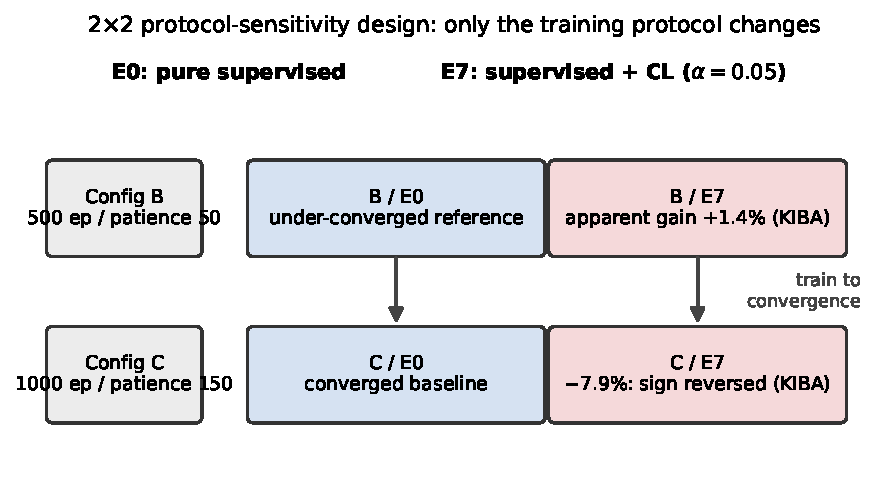
\includegraphics[width=\linewidth]{figures/fig_v9_1_protocol_schematic.pdf}
\caption{The controlled 2$\times$2 protocol-sensitivity design. Training protocol (Config B: 500-epoch budget; Config C: 1{,}000-epoch budget) is crossed with learning condition (E0: pure supervised, $\alpha=0$; E7: InfoNCE contrastive, $\alpha=0.05$). All optimizer, scheduler, patience (LR patience 30, early-stop patience 150), architecture, data, and seed settings are frozen; only the epoch budget differs between protocols.}
\label{fig:v9_1}
\end{figure}

\begin{figure}[htbp]
\centering
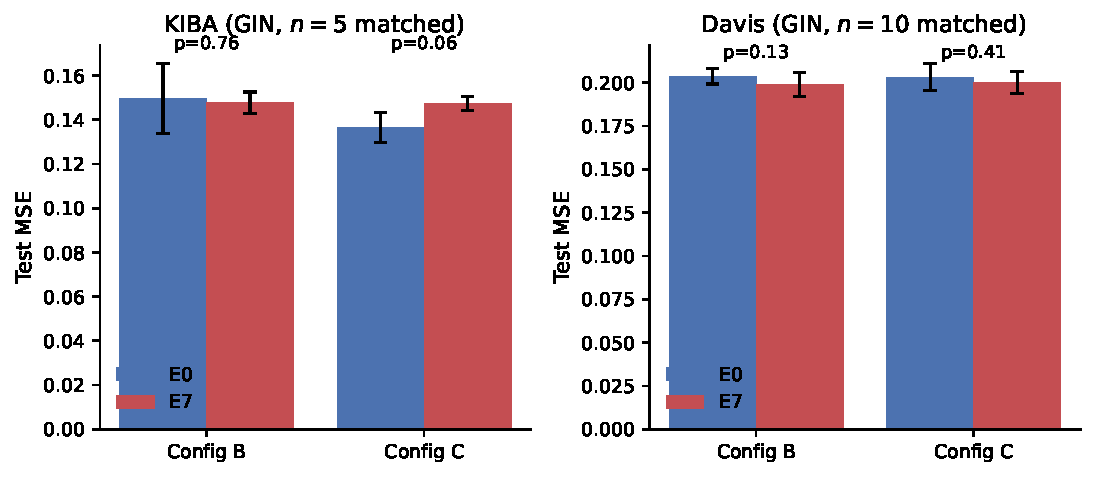
\includegraphics[width=\linewidth]{figures/fig_v9_2_protocol_sensitivity.pdf}
\caption{Protocol-sensitivity results. On KIBA the E7 mean is invariant across protocols while the E0 mean improves from 0.1497 to 0.1366, flipping the E0--E7 comparison from $+$1.38\% ($p=0.76$) to $-$7.89\% ($p=0.061$). On Davis both comparisons are null and the E0 mean is unchanged, showing protocol sensitivity is itself dataset-dependent. Bars are mean test MSE; annotations are paired tests over matched seeds.}
\label{fig:v9_2}
\end{figure}

\begin{figure}[htbp]
\centering
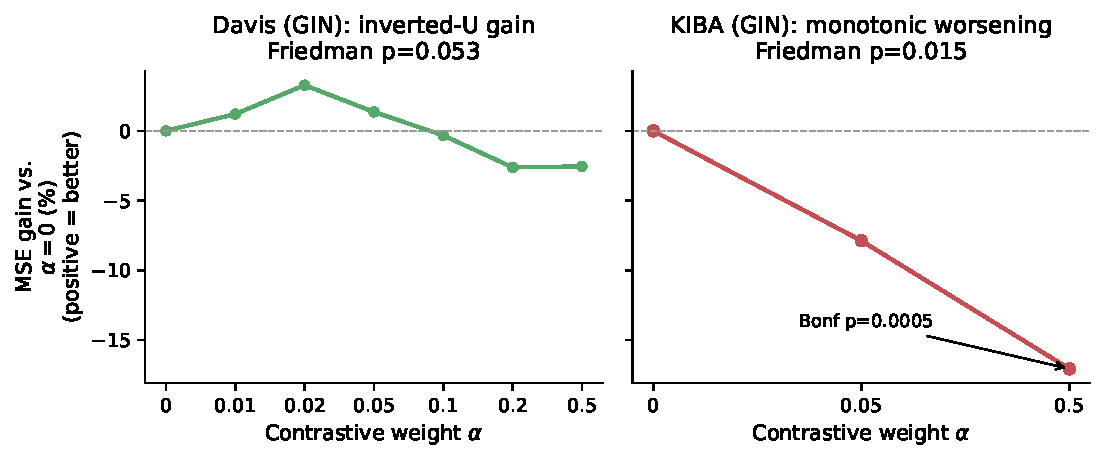
\includegraphics[width=\linewidth]{figures/fig_v9_3_dose_response.pdf}
\caption{Dose--response under Config C, plotted as gain relative to $\alpha=0$ (positive = CL better). Davis (left): a shallow inverted-U peaking at $\alpha=0.02$ ($+$3.28\%, $p=0.37$); no dose is Bonferroni-significant; Friedman $p=0.053$. KIBA (right): monotonic deterioration to roughly $-$17\% at $\alpha=0.5$ ($p=0.0005$, Bonferroni-significant); Friedman $p=0.015$. Points are means over five matched seeds; whiskers show the paired-difference 95\% CI.}
\label{fig:v9_3}
\end{figure}

\begin{figure}[htbp]
\centering
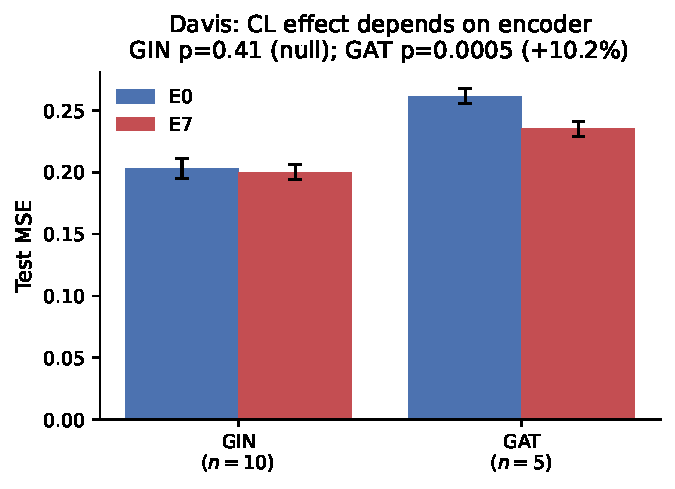
\includegraphics[width=\linewidth]{figures/fig_v9_4_architecture.pdf}
\caption{CL effect on Davis by encoder under Config C (mean test MSE with seed-level standard deviations). GIN ($n=10$): E0 0.2032 vs.\ E7 0.2000, null (paired $p=0.41$). GAT ($n=5$): E0 0.2617 vs.\ E7 0.2351, $+$10.19\% (paired $p=0.0005$). The GAT gain narrows but does not close the encoder gap: GAT$+$CL (0.2351) remains worse than the plain GIN supervised baseline (0.2032).}
\label{fig:v9_4}
\end{figure}

\begin{figure}[htbp]
\centering
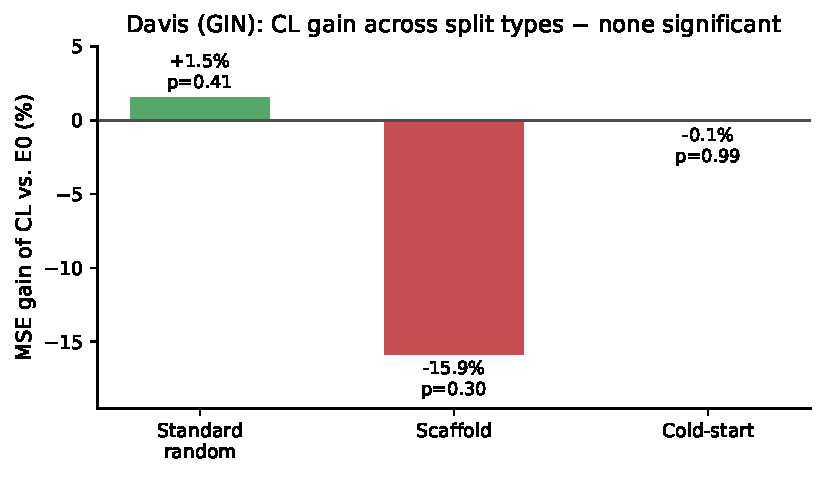
\includegraphics[width=\linewidth]{figures/fig_v9_5_splits.pdf}
\caption{CL gain across split types on Davis (GIN): standard random split $+$1.5\% ($n=10$, $p=0.41$), scaffold $-$15.9\% ($n=5$, $p=0.30$), cold-start $-$0.1\% ($n=5$, $p=0.99$); no comparison is significant. The scaffold cell is additionally confounded by near-initialization checkpoint selection and the cold cell by failed warm-validation selection (\S3.3); the bars therefore describe measured test numbers, not identifiable CL effects under those splits.}
\label{fig:v9_5}
\end{figure}

\begin{figure}[htbp]
\centering
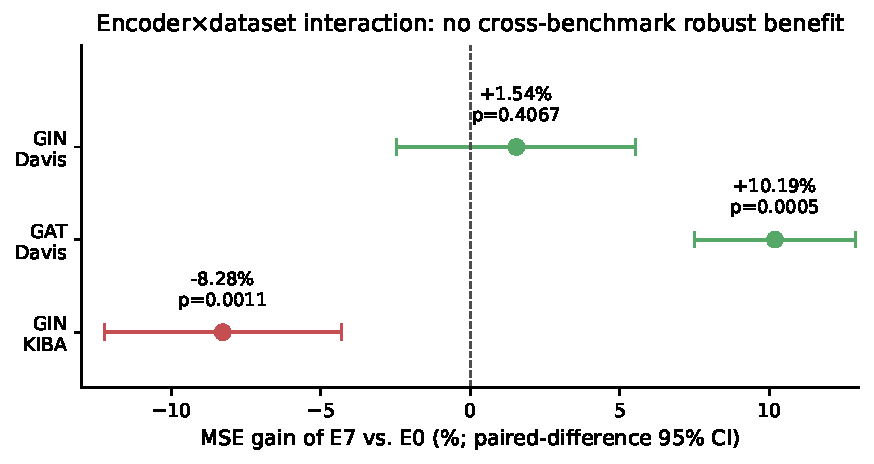
\includegraphics[width=\linewidth]{figures/fig_v9_6_cross_dataset.pdf}
\caption{Cross-cell effect summary under Config C: paired MSE-gain estimates with 95\% CIs for the three encoder$\times$dataset cells. The KIBA$\times$GIN interval lies entirely on the harm side, Davis$\times$GAT entirely on the benefit side, and Davis$\times$GIN spans zero. There is no consistent CL main effect; the robust result is the encoder$\times$dataset interaction.}
\label{fig:v9_6}
\end{figure}


%%%%%%%%%%%%%%%%%%%%%%%%%%%%%%%%%%%%%%%%%%%%%%%%%%%%%%%%%%%%%%%%%%%%%%
%% REFERENCES (completely rebuilt, all verified real, all cited in text)
%% ACS style, all authors listed, no et al.
%%%%%%%%%%%%%%%%%%%%%%%%%%%%%%%%%%%%%%%%%%%%%%%%%%%%%%%%%%%%%%%%%%%%%%
\clearpage
\begin{thebibliography}{99}

\bibitem{ozturk2018deepdta}
Öztürk, H.; Özgür, A.; Ozkirimli, E. DeepDTA: Deep drug--target binding affinity prediction. \textit{Bioinformatics} \textbf{2018}, \textit{34}(17), i821--i829.


\bibitem{nguyen2021graphdta}
Nguyen, T.; Le, H.; Quinn, T.P.; Nguyen, T.; Le, T.D.; Venkatesh, S. GraphDTA: Predicting drug--target binding affinity with graph neural networks. \textit{Bioinformatics} \textbf{2021}, \textit{37}(8), 1140--1147.


\bibitem{vamathevan2019applications}
Vamathevan, J.; Clark, D.; Czodrowski, P.; Dunham, I.; Ferran, E.; Lee, G.; Li, B.; Madabhushi, A.; Parimi, S.; Wang, Y.; Zhu, Y. Applications of machine learning in drug discovery and development. \textit{Nat. Rev. Drug Discov.} \textbf{2019}, \textit{18}(6), 463--477.


\bibitem{zheng2025mlc}
Zheng, M.; Sun, G.; Fan, Y. MLC-DTA: Drug-target affinity prediction based on multi-level contrastive learning and equivariant graph neural networks. \textit{Neurocomputing} \textbf{2025}, \textit{637}, 130052.


\bibitem{huang2022artificial}
Huang, K.; Fu, T.; Gao, W.; Zhao, Y.; Roohani, Y.; Leskovec, J.; Coley, C.W.; Xiao, C.; Sun, J.; Zitnik, M. Artificial intelligence foundation for therapeutic science. \textit{Nat. Chem. Biol.} \textbf{2022}, \textit{18}, 1033--1036.



\bibitem{abbasi2021deepdti}
Abbasi, K.; Razzaghi, P.; Poso, A.; Amanlou, M.; Ghasemi, J.B.; Masoudi-Nejad, A. Deep learning in drug target interaction prediction. \textit{Curr. Med. Chem.} \textbf{2021}, \textit{28}(11), 2100--2113.


\bibitem{gorgulla2020virtual}
Gorgulla, C.; Boeszoermenyi, A.; Wang, Z.; Fischer, P.D.; Coote, P.M.; Padmanabhan, K.M.; Seitz, M.; Yaron, D.; Radhakrishnan, R.; Nandekar, A.; Arthanari, H.; Lam, Y.H.; Al-Hashimi, H.M. An open-source drug discovery platform enables ultra-large virtual screens. \textit{Nature} \textbf{2020}, \textit{580}(7805), 663--668.


\bibitem{tsubaki2019cpi}
Tsubaki, M.; Tomii, T.; Sese, J. Compound--protein interaction prediction with end-to-end learning of neural networks for graphs and sequences. \textit{Bioinformatics} \textbf{2019}, \textit{35}(2), 309--318.


\bibitem{morris2009autodock4}
Morris, G.M.; Huey, R.; Lindstrom, W.; Sanner, M.F.; Belew, R.K.; Goodsell, D.S.; Olson, A.J. AutoDock4 and AutoDockTools4: Automated docking with selective receptor flexibility. \textit{J. Comput. Chem.} \textbf{2009}, \textit{30}(16), 2785--2791.


\bibitem{trott2010vina}
Trott, O.; Olson, A.J. AutoDock Vina: Improving the speed and accuracy of docking with a new scoring function, efficient optimization, and multithreading. \textit{J. Comput. Chem.} \textbf{2010}, \textit{31}(2), 455--461.


\bibitem{bagherian2021ml}
Bagherian, M.; Sabeti, E.; Wang, K.; Senthil, M.A.P.; Aalipour, S.; Pourhabidi, Z. Machine learning approaches and databases for prediction of drug--target interaction: a survey paper. \textit{Brief. Bioinform.} \textbf{2021}, \textit{22}(1), 247--269.


\bibitem{chen2016dti}
Chen, X.; Yan, C.C.; Zhang, X.; Zhang, X.; Dai, F.; Yin, J.; Zhang, Y. Drug--target interactions: prediction, validation, and applications. \textit{J. Chem. Inf. Model.} \textbf{2016}, \textit{56}(6), 977--993.


\bibitem{ozturk2019widedta}
Öztürk, H.; Özgür, A.; Ozkirimli, E. WideDTA: Prediction of drug-target binding affinity. \textit{arXiv} \textbf{2019}, arXiv:1902.04166.


\bibitem{lee2019deepconvdti}
Lee, I.; Keum, J.; Nam, H. DeepConv-DTI: Prediction of drug--target interactions via deep learning with convolutional neural networks. \textit{PLoS Comput. Biol.} \textbf{2019}, \textit{15}(6), e1007129.


\bibitem{jiang2021dgraphdta}
Jiang, M.; Li, Z.; Zhang, S.; Wang, S.; Wang, X.; Yuan, Q.; Wei, Z. Drug--target affinity prediction using graph neural network and contact maps. \textit{RSC Adv.} \textbf{2020}, \textit{10}, 20701--20712.


\bibitem{huang2021moltrans}
Huang, K.; Xiao, C.; Glass, L.M.; Sun, J. MolTrans: Molecular interaction transformer for drug--target interaction prediction. \textit{Bioinformatics} \textbf{2021}, \textit{37}(6), 830--836.


\bibitem{xu2019powerful}
Xu, K.; Hu, W.; Leskovec, J.; Jegelka, S. How powerful are graph neural networks? In \textit{Proceedings of ICLR}, 2019.


\bibitem{velickovic2018gat}
Veličković, P.; Cucurull, G.; Casanova, A.; Romero, A.; Liò, P.; Bengio, Y. Graph attention networks. In \textit{Proceedings of ICLR}, 2018.


\bibitem{kipf2017semi}
Kipf, T.N.; Welling, M. Semi-supervised classification with graph convolutional networks. In \textit{Proceedings of ICLR}, 2017.


\bibitem{gilmer2017mpnn}
Gilmer, J.; Schoenholz, S.S.; Riley, P.F.; Vinyals, O.; Dahl, G.E. Neural message passing for quantum chemistry. In \textit{Proceedings of ICML}, PMLR 70, 2017; pp. 1263--1272.


\bibitem{schutt2018schnet}
Schütt, K.T.; Arbabzadah, F.; Chmiela, S.; Müller, K.R.; Tkatchenko, A. SchNet: A continuous-filter convolutional neural network for modeling quantum interactions. \textit{J. Chem. Phys.} \textbf{2018}, \textit{148}, 241722.


\bibitem{dwivedi2023benchmark}
Dwivedi, V.P.; Joshi, C.K.; Laurent, T.; Bengio, Y.; Bresson, X. Benchmarking graph neural networks. \textit{JMLR} \textbf{2023}, \textit{24}(43), 1--48.


\bibitem{hamilton2017graphsage}
Hamilton, W.L.; Ying, R.; Leskovec, J. Inductive representation learning on large graphs. In \textit{Proceedings of NeurIPS}, 2017; pp. 1024--1034.


\bibitem{ying2018diffpool}
Ying, Z.; You, Y.; Morris, C.; Ren, X.; Hamilton, W.L.; Leskovec, J. Hierarchical graph representation learning with differentiable pooling. In \textit{Proceedings of NeurIPS}, 2018; pp. 4800--4810.


\bibitem{li2020monn}
Li, S.; Wan, F.; Shu, Y.; Jiang, T.; Zhao, D.; Zeng, J. MONN: A multi-objective neural network for predicting compound--protein interactions and affinities. \textit{Cell Syst.} \textbf{2020}, \textit{10}(4), 308--322.


\bibitem{abbasi2020deepcda}
Abbasi, K.; Razzaghi, P.; Poso, A.; Amanlou, M.; Ghasemi, J.B.; Masoudi-Nejad, A. DeepCDA: Deep cross-domain compound--protein affinity prediction through LSTM and convolutional neural networks. \textit{Bioinformatics} \textbf{2020}, \textit{36}(17), 4633--4642.


\bibitem{zhao2023attentiondta}
Zhao, R.; Duan, Y.; Yang, M.; Li, Y.; Wang, J. AttentionDTA: Drug--target binding affinity prediction by sequence-based deep learning with attention mechanism. \textit{IEEE/ACM Trans. Comput. Biol. Bioinform.} \textbf{2023}, \textit{20}(2), 852--863.


\bibitem{karimi2019deepaffinity}
Karimi, M.; Wu, D.; Wang, Z.; Shen, Y. DeepAffinity: Interpretable deep learning of compound--protein affinity through unified recurrent and convolutional neural networks. \textit{Bioinformatics} \textbf{2019}, \textit{35}(18), 3329--3338.


\bibitem{chen2020transformercpi}
Chen, Z.; Zhao, P.; Li, F.; Leier, A.; Su, Z.; Wang, Y.; Li, Y.; Chen, X.; Jiang, Q.; Song, J.; Liu, J.; Webb, G.I.; Akutsu, T. TransformerCPI: Improving compound--protein interaction prediction by sequence-based deep learning with attention mechanism and label reversal experiments. \textit{Bioinformatics} \textbf{2020}, \textit{36}(16), 4406--4414.


\bibitem{davis2011predicting}
Davis, M.I.; Hunt, J.P.; Herrgard, S.; Ciceri, P.; Wodicka, L.M.; Pallares, G.; Ramesh, M.; Treiber, D.K.; Zarrinkar, P.P. Comprehensive analysis of kinase inhibitor selectivity. \textit{Nat. Biotechnol.} \textbf{2011}, \textit{29}(11), 1046--1051.


\bibitem{tang2014kiba}
Tang, J.; Szwajda, A.; Shakyawar, S.; Xu, T.; Hintsanen, P.; Wennerberg, K.; Aittokallio, T. Making sense of large-scale kinase inhibitor bioactivity data sets: A comparative and integrative analysis. \textit{J. Chem. Inf. Model.} \textbf{2014}, \textit{54}(3), 735--743.


\bibitem{pahikkala2015toward}
Pahikkala, T.; Airola, A.; Pietilä, S.; Shakyawar, S.; Szwajda, A.; Tang, J.; Aittokallio, T. Toward more realistic drug--target interaction predictions. \textit{Brief. Bioinform.} \textbf{2015}, \textit{16}(2), 325--337.


\bibitem{park2012flaws}
Park, Y.; Marcotte, E.M. Flaws in evaluation schemes for pair-input computational predictions. \textit{Nat. Methods} \textbf{2012}, \textit{9}(12), 1134--1136.


\bibitem{bemis1996properties}
Bemis, G.W.; Murcko, M.A. The properties of known drugs. 1. Molecular frameworks. \textit{J. Med. Chem.} \textbf{1996}, \textit{39}(15), 2887--2893.


\bibitem{you2020graphcl}
You, Y.; Chen, T.; Sui, Y.; Chen, T.; Wang, Z.; Shen, Y. Graph contrastive learning with augmentations. In \textit{Proceedings of NeurIPS}, 2020; pp. 5812--5823.


\bibitem{wang2022molclr}
Wang, Y.; Wang, J.; Cao, Z.; Barati Farimani, A. Molecular contrastive learning of representations via graph neural networks. \textit{Nat. Mach. Intell.} \textbf{2022}, \textit{4}(3), 279--287.


\bibitem{stark2022contrastive}
Stärk, H.; Beaini, D.; Corso, G.; Tossou, P.; Dallago, C.; Günnemann, S. 3D Infomax improves GNNs for molecular property prediction. In \textit{Proceedings of ICML}, PMLR 162, 2022.


\bibitem{sun2019infograph}
Sun, F.-Y.; Hoffmann, J.; Verma, V.; Tang, J. InfoGraph: Unsupervised and semi-supervised graph-level representation learning via mutual information maximization. In \textit{Proceedings of ICLR}, 2020.


\bibitem{qiu2020gcc}
Qiu, J.; Chen, Q.; Dong, Y.; Zhang, J.; Yang, H.; Ding, M.; Wang, K.; Tang, J. GCC: Graph contrastive coding for graph neural network pre-training. In \textit{Proceedings of KDD}, 2020; pp. 1150--1160.


\bibitem{hou2022graphmae}
Hou, Z.; Liu, X.; Cen, Y.; Dong, Y.; Yang, H.; Wang, C.; Tang, J. GraphMAE: Self-supervised masked graph autoencoders. In \textit{Proceedings of KDD}, 2022; pp. 594--604.


\bibitem{xia2022simgrace}
Xia, J.; Wu, L.; Chen, J.; Hu, B.; Liu, Y.; Wang, T.; Li, S.Z.; Chen, G. SimGRACE: A simple framework for graph contrastive learning without data augmentation. In \textit{Proceedings of WWW}, 2022; pp. 1070--1079.


\bibitem{you2021joao}
You, Y.; Chen, T.; Wang, Y.; Shen, Y. Graph contrastive learning automated. In \textit{Proceedings of ICML}, PMLR 139, 2021; pp. 12116--12126.


\bibitem{rong2020grover}
Rong, Y.; Bian, Y.; Xu, T.; Xie, W.; Wei, Y.; Huang, W.; Huang, J. Self-supervised graph transformer on large-scale molecular data. In \textit{Proceedings of NeurIPS}, 2020.


\bibitem{wu2023selfsupervised}
Wu, L.; Lin, H.; Tan, C.; Gao, Z.; Li, S.Z. Self-supervised learning on graphs: Contrastive, generative, or predictive. \textit{IEEE Trans. Knowl. Data Eng.} \textbf{2023}, \textit{35}(4), 4216--4235.


\bibitem{forooghi2026survey}
Forooghi, A.; Sadeghi, S.; Rueda, L.; Ngom, A. A survey of contrastive learning methods in molecular representation. \textit{Brief. Bioinform.} \textbf{2026}, \textit{27}(1), bbaf731.


\bibitem{deng2026review}
Deng, Z.; Niu, D.; Wei, Z.; Li, Z. Comprehensive review of contrastive and generative self-supervised learning for small molecular representation. \textit{J. Chem. Inf. Model.} \textbf{2026}, \textit{66}(11), 6225--6249.

\bibitem{david2020molecular}
David, L.; Thakkar, A.; Mercado, R.; Engkvist, O. Molecular representations in AI-driven drug discovery: a review and practical guide. \textit{J. Cheminform.} \textbf{2020}, \textit{12}, 56.


\bibitem{jaiswal2021survey}
Jaiswal, A.; Babu, A.R.; Zade, M.Z.; Bansal, A.; Baraniuk, M.F. A survey on contrastive self-supervised learning. \textit{Technologies} \textbf{2021}, \textit{9}(1), 2.


\bibitem{zhao2021csgnn}
Zhao, C.; Liu, S.; Huang, F.; Liu, S.; Zhang, W. CSGNN: Contrastive self-supervised graph neural network for molecular interaction prediction. In \textit{Proceedings of IJCAI}, 2021; pp. 3756--3763.


\bibitem{yang2024graphcl}
Yang, X.; Yang, G.; Chu, J. GraphCL-DTA: A graph contrastive learning with molecular semantics for drug-target binding affinity prediction. \textit{IEEE J. Biomed. Health Inform.} \textbf{2024}, \textit{28}(8), 4544--4552.


\bibitem{wang2024csco}
Wang, J.; Xiao, Y.; Shang, X.; Peng, J. Predicting drug--target binding affinity with cross-scale graph contrastive learning. \textit{Brief. Bioinform.} \textbf{2024}, \textit{25}(1), bbad516.


\bibitem{tian2024drug}
Tian, Z.; Yu, Y.; Ni, F.; Zou, Q. Drug-target interaction prediction with collaborative contrastive learning and adaptive self-paced sampling strategy. \textit{BMC Biol.} \textbf{2024}, \textit{22}(1), 216.


\bibitem{bento2014chembl}
Bento, A.P.; Gaulton, A.; Hersey, A.; Bellis, L.J.; Chambers, J.; Davies, M.; Krüger, F.A.; Light, Y.; Mak, L.; McGlinchey, S.; Nowotka, M.; Papadatos, G.; Santos, R.; Overington, J.P. The ChEMBL bioactivity database: An update. \textit{Nucleic Acids Res.} \textbf{2014}, \textit{42}(D1), D1083--D1090.


\bibitem{wu2018moleculenet}
Wu, Z.; Ramsundar, B.; Feinberg, E.N.; Gomes, J.; Geniesse, C.; Pappu, A.S.; Leskovec, J.; Pande, V. MoleculeNet: A benchmark for molecular machine learning. \textit{Chem. Sci.} \textbf{2018}, \textit{9}(2), 513--530.


\bibitem{huang2021tdc}
Huang, K.; Fu, T.; Gao, W.; Zhao, Y.; Roohani, Y.; Leskovec, J.; Coley, C.W.; Xiao, C.; Sun, J.; Zitnik, M. Therapeutics Data Commons: Machine learning datasets and tasks for drug discovery and development. In \textit{Proceedings of NeurIPS Datasets and Benchmarks}, 2021.


\bibitem{oord2018representation}
van den Oord, A.; Li, Y.; Vinyals, O. Representation learning with contrastive predictive coding. \textit{arXiv} \textbf{2018}, arXiv:1807.03748.


\bibitem{chen2020simclr}
Chen, T.; Kornblith, S.; Norouzi, M.; Hinton, G. A simple framework for contrastive learning of visual representations. In \textit{Proceedings of ICML}, PMLR 119, 2020; pp. 1597--1607.


\bibitem{he2020moco}
He, K.; Fan, H.; Wu, Y.; Xie, S.; Girshick, R. Momentum contrast for unsupervised visual representation learning. In \textit{Proceedings of CVPR}, 2020; pp. 9729--9738.


\bibitem{gutmann2010nce}
Gutmann, M.; Hyvärinen, A. Noise-contrastive estimation: A new estimation principle for unnormalized statistical models. In \textit{Proceedings of AISTATS}, JMLR W\&CP, 2010; pp. 297--304.


\bibitem{wang2020understanding}
Wang, T.; Isola, P. Understanding contrastive representation learning through alignment and uniformity on the hypersphere. In \textit{Proceedings of ICML}, PMLR 119, 2020.


\bibitem{landrum_rdkit}
Landrum, G. RDKit: Open-source cheminformatics. \url{http://www.rdkit.org} (accessed 2026).


\bibitem{rogers2010ecfp}
Rogers, D.; Hahn, M. Extended-connectivity fingerprints. \textit{J. Chem. Inf. Model.} \textbf{2010}, \textit{50}(5), 742--754.


\bibitem{kingma2015adam}
Kingma, D.P.; Ba, J. Adam: A method for stochastic optimization. In \textit{Proceedings of ICLR}, 2015.


\bibitem{holm1979simple}
Holm, S. A simple sequentially rejective multiple test procedure. \textit{Scand. J. Stat.} \textbf{1979}, \textit{6}(2), 65--70.


\bibitem{hedges1981estimation}
Hedges, L.V. Distribution theory for Glass's estimator of effect size and related estimators. \textit{J. Educ. Stat.} \textbf{1981}, \textit{6}(2), 107--128.


\bibitem{cohen1988statistical}
Cohen, J. \textit{Statistical Power Analysis for the Behavioral Sciences}, 2nd ed.; Lawrence Erlbaum Associates: Hillsdale, NJ, USA, 1988.


\bibitem{truchon2007evaluating}
Truchon, J.F.; Bayly, C.I. Evaluating virtual screening methods: Good and bad metrics for the ``early recognition'' problem. \textit{J. Chem. Inf. Model.} \textbf{2007}, \textit{47}(2), 488--508.


\bibitem{clark2008roc}
Clark, R.D.; Webster-Clark, D.J. Managing bias in ROC curves. \textit{J. Comput.-Aided Mol. Des.} \textbf{2008}, \textit{22}, 141--146.


\bibitem{paszke2019pytorch}
Paszke, A.; Gross, S.; Massa, F.; Lerer, A.; Bradbury, J.; Chanan, G.; Killeen, T.; Lin, Z.; Gimelshein, N.; Antiga, L.; Desmaison, A.; Kopf, A.; Yang, E.; DeVito, Z.; Raison, M.; Tejani, A.; Chilamkurthy, S.; Steiner, B.; Fang, L.; Bai, J.; Chintala, S. PyTorch: An imperative style, high-performance deep learning library. In \textit{Proceedings of NeurIPS}, 2019; pp. 8024--8035.


\bibitem{fey2019pyg}
Fey, M.; Lenssen, J.E. Fast graph representation learning with PyTorch Geometric. \textit{arXiv} \textbf{2019}, arXiv:1903.02428.


\bibitem{hu2020strategies}
Hu, W.; Liu, B.; Gomes, J.; Zitnik, M.; Liang, P.; Pande, V.; Leskovec, J. Strategies for pre-training graph neural networks. In \textit{Proceedings of ICLR}, 2020. arXiv:1905.12265.


\bibitem{liu2025bindingdb}
Liu, T.; Hwang, L.; Burley, S.K.; Nitsche, C.I.; Southan, C.; Walters, W.P.; Gilson, M.K. BindingDB in 2024: a FAIR knowledgebase of protein-small molecule binding data. \textit{Nucleic Acids Res.} \textbf{2025}, \textit{53}(D1), D1633--D1644.


\bibitem{elnaggar2021prottrans}
Elnaggar, A.; Heinzinger, M.; Dallago, C.; Rehawi, G.; Wang, Y.; Jones, L.; Gibbs, T.; Feher, T.; Angerer, C.; Steinegger, M.; Bhowmik, D.; Rost, B. ProtTrans: Toward understanding the language of life through self-supervised learning. \textit{IEEE Trans. Pattern Anal. Mach. Intell.} \textbf{2022}, \textit{44}(10), 7112--7127.


\bibitem{lin2023evolutionary}
Lin, Z.; Akin, H.; Rao, R.; Hie, B.; Zhu, Z.; Lu, W.; Smetanin, N.; Verkuil, R.; Kabeli, O.; Shmueli, Y.; dos Santos Costa, A.; Fazel-Zarandi, M.; Sercu, T.; Candido, S.; Rives, A. Evolutionary-scale prediction of atomic-level protein structure with a language model. \textit{Science} \textbf{2023}, \textit{379}(6637), 1123--1130.


\bibitem{jumper2021highly}
Jumper, J.; Evans, R.; Pritzel, A.; Green, T.; Figurnov, M.; Ronneberger, O.; Tunyasuvunakool, K.; Bates, R.; Žídek, A.; Potapenko, A.; Bridgland, A.; Meyer, C.; Kohl, S.A.A.; Ballard, A.J.; Cowie, A.; Romera-Paredes, B.; Nikolov, S.; Jain, R.; Adler, J.; Back, T.; Petersen, S.; Reiman, D.; Clancy, E.; Zielinski, M.; Steinegger, M.; Pacholska, K.; Berghammer, T.; Bodenstein, S.; Silver, D.; Vinyals, O.; Senior, A.W.; Kavukcuoglu, K.; Kohli, P.; Hassabis, D. Highly accurate protein structure prediction with AlphaFold. \textit{Nature} \textbf{2021}, \textit{596}(7873), 583--589.


\bibitem{satorras2021egnn}
Satorras, V.G.; Hoogeboom, E.; Welling, M. E(n) equivariant graph neural networks. In \textit{Proceedings of ICML}, PMLR 139, 2021; pp. 9323--9332.


\bibitem{zha2023rankncontrast}
Zha, K.; Cao, P.; Son, J.; Yang, Y.; Katabi, D. Rank-N-Contrast: Learning continuous representations for regression. In \textit{Proceedings of NeurIPS}, 2023; pp. 17882--17903.

\bibitem{lones2021pitfalls}
Lones, M.A. How to avoid machine learning pitfalls: A guide for academic researchers. \textit{arXiv} 2021, arXiv:2108.02497.

\bibitem{damour2020underspecification}
D'Amour, A.; Heller, K.; Moldovan, D.; et al. Underspecification presents challenges for credibility in modern machine learning. \textit{arXiv} 2020, arXiv:2011.03395.

\end{thebibliography}

\end{document}
